\section{Biological}
\newcommand{\salmonellatyphii}{\textit{Salmonella typhii}}
\newcommand{\campylobacter}{\textit{Campylobacter}}

This chapter provides an overview of the problem that clustering for \bslong{} and \kraplong{} attempts to solve.
Fecal contamination is a serious health concern that public officials work hard to mitigate effects of.
\MSTlong{} is a solution typically that these officials typically employ in order to discover the source of fecal contamination and avert more contamination.
Bacterial strain typing is just one of these techniques that \cploplong{} employs in a cost-effective manner.

\subsection{Fecal Contamination}
Fecal contamination is dangerous for humans and animals alike.
Pathogenic bacteria reside in fecal matter and contamination of publicly accessible and environmental water sources expose humans and animals to their dangerous effects.
Often, it is up to natural resource managers and public health officials to both eliminate and prevent fecal contamination from occurring.
Preventing contact with such bacteria is key to maintaining good public and environmental health.

Fecal matter can contain many different types of microbes, some of which are pathogenic.
A \textit{pathogen} is a microbe that causes disease in an animal.
\index{pathogen}
Pathogenic microbes that make their way into fecal matter include \ecolilong{} (\ecoli{}), \salmonellatyphii{}, and \campylobacter{}.
Diseases they might cause can include nose and ear infections, dysentary, and typhoid fever.
Zoonotic pathogens --- those that wild animals, pets, or livestock can transmit to humans --- are of particular concern, since it can be challenging to determine the source of the contamination.
The use of antibiotics in livestock increases the resistance of some pathogens to traditional therapeutic techniques to treat the disease in humans \cite{rogers2005detecting}.
It behooves public health officials and natural resource managers alike to mitigate the cause of fecal contamination for the safey and health of the public.

\subsection{\MSTlong{} with \FIBlong{}}
\MSTlong{} (\mst{}) aims to discover the \spec{} of microbial lifeforms, often employing \FIBlong{} (\fib{}) to discover the source of fecal contamination.
Many techniques exist that leverage unique characteristics of the \fib{} present in the fecal matter.
Ultimately, choosing the right \fib{} requires that researchers and investigators understand their resource and budget constraints, and tailor their \mst{} process accordingly.

\mst{} techniques using \fib{} generally fall into two broad categories: library-dependent and library-independent.
Certain \fib{} and bacteriophages are known to be from specific \spec{}, making \spec{} assessment of fecal matter possible without the need to build a library.
However, most library-independent \mst{} cannot establish a \spec{} source ``beyond humans and a few domestic species'' \cite{rogers2005detecting}.

Library-dependent techniques build a library of known \spec{} samples of \fib{} and uses this data to determine \spec{} for an unknown sample.
The effort needed to build such a library can be considerable, often requiring the genetic sequencing of a considerate number of samples to be effective \cite{rogers2005detecting}.
Commonly, these libraries are only useful for the environment in which the researchers sampled from.
What they gain by building such a library is the flexibility to determine the source of fecal matter from multiple \spec{} \cite{rogers2005detecting}.
These library-dependent techniques rely on the of bacterial strain typing, discusses in the following section.


\subsection{Delineating Bacterial Strains}
When using \fib{} for \mst{}, distinguishing between \bslongs{} (\bs{}) is a dynamic tool that can allow researchers to determine the source of fecal matter from a variety of \spec{}.
Other methods that rely on \mst{} are usually limited in the \spec{} they are effective at sourcing.
By building a library of \fib{} samples, investigators can leverage bacterial strain typing to create a flexible and widely applicable method of sourcing fecal matter.
Nevertheless, it has some drawbacks that, with some effort, \mst{} investigators and researchers can overcome.

Bacterial strain typing for \mst{} relies on the notion that strains of \fib{} remain mostly unique to the \spec{} from which they came.
A \textit{strain} of a species of microbe is a subtype of that species where the microbes in that strain are closely related to each other in some meaningful way. 
\index{strain}
Generally, how one defines a strain differs between research groups, as each definition of a strain depends on the characterization of the microbe in question and the methods used to derive such characterizations.
A strain, then, can be thought of as consisting of individuals descending from the same individual to generate a ``group'' or ``family.''

\ecolilong{} (\ecoli{}) inhabits the gut of many animals, but only certain strains are pathogenic.
The guts of animals and humans are a great environment for flora like \ecoli{} to thrive and multiply.
\ecoli{} can get into the gut in many ways based on the environment the \host{} lives in, the food they eat, and the other animals they interact with.
Since \ecoli{} resides in so many different species, researchers typically use it as the \fib{} of choice for library-based \mst{}.

As \cite{rogers2005detecting} points out, the strains in \ecoli{} can change considerably  within the same \spec{}.
Geography, time, rainfall, and habitat all can have an effect on the strains present in a particular \spec{} and even \host{}.
The transient nature of some \ecoli{} strains forces researchers to build a library that contains a considerable number of samples to encapsulate the full spread of strains in the relevant \spec{}, adding to the cost and efforts needed to perform \mst{} and usually limiting the environmental scope of the library built to the environment in which it was sampled from.
\cploplong{} attempts to remedy this by building a cheap yet reliable method of distinguishing between strains using \pyros{} on the two \itsshort{} regions of \ecoli{}.

\section{\cplop{} Makeup}
\autoref{fig:species} shows the distribution of \cplop{} \isols{} considered in this study among its 53 different \spec{}.
\begin{figure}[t]
    \centering
    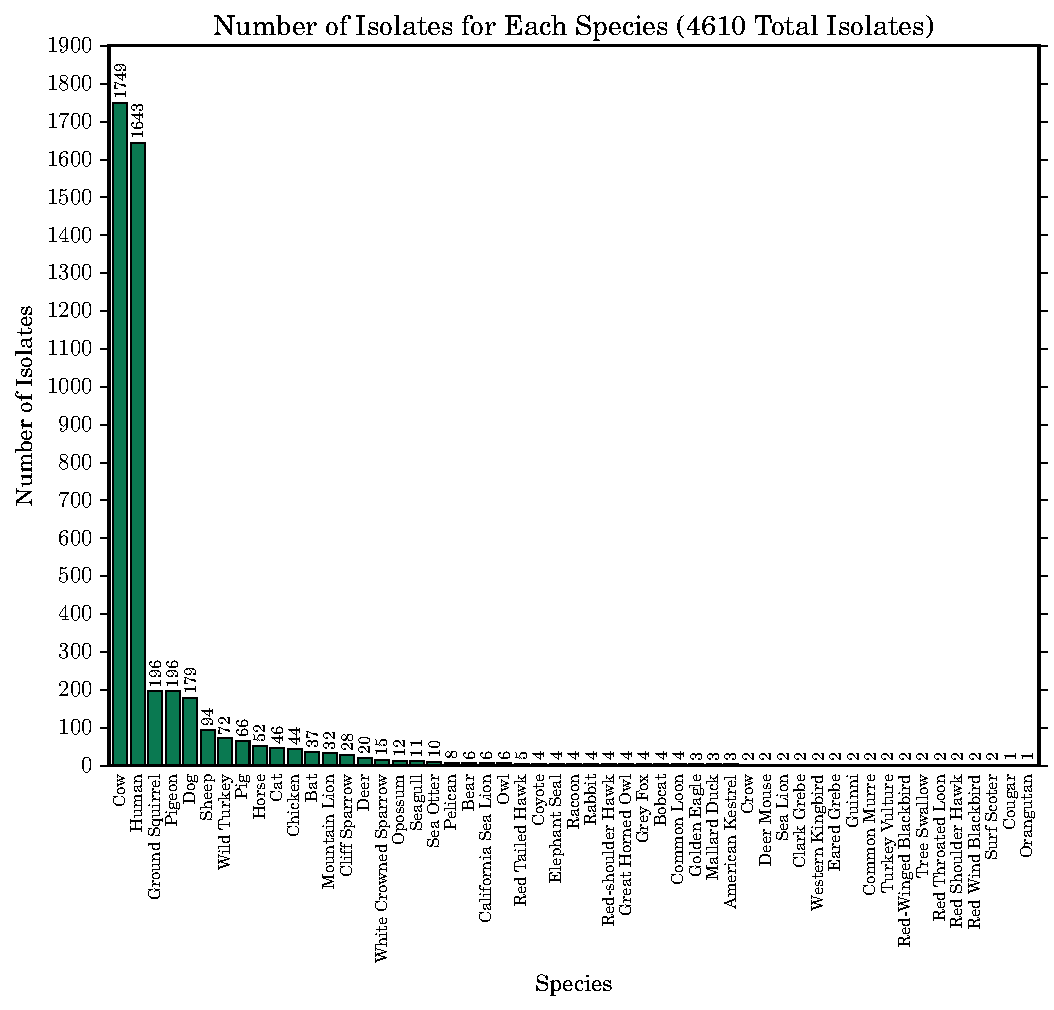
\includegraphics[width=\linewidth]{figures/bs/species_hist.pdf}
    \caption{
    A histogram of the number of \isols{} of each species in our study, taken from \cplop{}.
    There are 4,610 total \isols{} from 53 different \specs{}.}
    \label{fig:species}
\end{figure}

There are a total of 4,610 \isols{} in our dataset\footnote{A simplified version of \cplop{} containing \isol{} IDs, \spec{}, and \zscore{}s can be found at \texttt{https://github.com/jmcgover/cplop-acm-bcb-2016}.}. As seen from Figure \ref{fig:species},
the organic growth of \cplop{} yielded disproportionately many \ecoli{} isolates originating
from humans and cows (however, as shall be seen below, these isolates belong to a large number of strains). Each \isol{} is represented in \cplop{} with two \pyros{} ---  one each for \its{1} and \its{2} 
region.